\documentclass[twocolumn]{article}
\usepackage[utf8]{inputenc}
\usepackage{graphicx}
\usepackage[]{algorithm}
\usepackage{algpseudocode}
\usepackage{tikz}
\usetikzlibrary{positioning}
\graphicspath{{./images/}}

\title{Étude d'un algorithme génétique sur le problème one-max}
\author{BOKA Yao }
\date{Novembre 2018}

\begin{document}

\maketitle

\section{Introduction}

Les problèmes d'optimisation peuvent être divisés en deux grandes catégories. On parle d'\emph{optimisation continue} lorsque les variables manipulées sont continues et l'on parle d'\emph{optimisation combinatoire} lorsque les variables manipulées sont discrètes.
Pour un problème combinatoire donné, l'optimisation consiste à trouver une solution optimale dans un  ensemble de solutions possibles.  
Les \emph{Algorithmes Evolutionnaires} font partie des méthodes d'optimisation stochastiques, inspirés des processus biologiques et particulièrement des théories darwiniennes  selon lesquelles un ensemble d'organismes biologiques subissent des processus et pressions environnementaux qui leurs permettent de mieux s'adapter à environnement. Il existe plusieurs variantes de ces algorithmes parmi lesquelles on peut citer les \emph{stratégies d'évolution}, la \emph{programmation évolutionnaire}, \emph{les algorithmes génétiques} et la \emph{programmation génétique}...
Le principe général d'un algorithme évolutionnaire est le suivant: On part d'un ensemble de solutions candidates générées/obtenues aléatoirement représentées par une  \emph{population}, on sélectionne au fil des générations (représentées par un certains nombre d'itérations) des individus parents de la population sur lesquels sont appliqués les opérateurs variations que sont le \emph{croisement} et/ou les \emph{mutations}. Le croisement est un opérateur qui consiste à combiner deux ou plusieurs individus parents afin d'obtenir un ou plusieurs nouveaux individus enfants. La mutation est une opérateur de modification qui s'applique sur un individu enfant. Les nouveaux individus enfants sont par la suite intégrés dans la population par remplacement de certains individus déjà présents dans la population. Ce principe est représenté par le schéma dans la figure 1.

\begin{figure}[h]
    \centering
    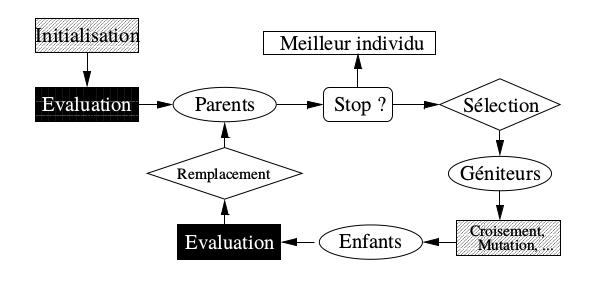
\includegraphics[width=0.5\textwidth]{schema_EA}{\centering}
    \caption{Schéma d'un Algorithme Evolutionnaire}
    \label{fig:mesh1}
\end{figure}

Les différentes variantes d'un algorithme évolutionnaire suivent ce même schéma mais diffèrent de l'espace de recherche (l'espace sur lequel est défini la fonction objectif), de la représentation du problème et de la définition des opérateurs de variations.

\section{L'algorithme génétique Steady State}
\subsection{ Présentation}
Les algorithmes génétiques (AG) ont été introduits en 1975 par John Holland et imaginés comme outils de modélisation de l'adaptation. On les caractérise principalement par la représentation du génotype de façon binaire (i.e un individu est représenté par une chaîne de bit).  L'algorithme 1 présenté ci-dessous  présente un  pseudo-code de l'algorithme selon le schéma \emph{Steady State}.

\begin{algorithm}
\caption{Pseudo-code d'un Algorithme Génétique Steady State}
\begin{algorithmic}[1]
\State $P\gets initPop(P)$ //Initialisation
\State evalPop($P$) //Évaluation 
\While {le critère d'arrêt n'est pas respecté}
    \State // Sélection
    \State $parents \gets selectionFrom(P$)
    \State // Croisement
    \State $enfants\gets croisement(parents, p_c)$ 
    \State //Mutation
    \State $enfants\gets mutation(enfants, p_m)$
    \State // Évaluation
    \State evalPop($P$)
    \State // Insertion/remplacement
    \State $P\gets insertionTo(enfants,P)$ 
\EndWhile
\end{algorithmic}
\end{algorithm}

\subsection{Les composants de l'algorithme}

Un individu est représenté comme une chaîne de bits de taille $n$.
La fonction de \emph{fitness} $f$ : permet de calculer le nombre de 1 que contient un individu $I$. Exemple: avec $I= 1100101, f(I) = 4.$
	
\paragraph{Initialisation:}
Plusieurs choix se présentent tels que partir d'une population de $n$ individus dont tous les $n$ bits constituant la chaîne sont initialisés à $0$, ou partir d'une population de $p$ individus dont la valeur des bits de sa structure générée de façon aléatoire. Seule la première méthode d'initialisation a été utilisée dans notre étude.
\paragraph{La sélection:}
Dans le cadre de ce travail, 3 méthodes sont utilisées: 
La sélection\emph{best}: qui consiste à choisir dans la population les deux meilleurs, (ie la meilleure évaluation selon $f$).
La sélection\emph{ aléatoire}: qui consiste à choisir de façon aléatoire deux individus dans la population.
La sélection par \emph{tournoi} : qui consiste à sélectionner $t$ individus de façon aléatoire et d'en choisir les deux meilleurs.

\paragraph{La récombinaison/croisement}:
Le \emph{croisement mono-point}: Consiste à déterminer aléatoirement un point de croisement, ce qui permet de croiser les parties des deux parents afin d'obtenir les deux individus enfants.
Le croisement \emph{uniforme:} Consistent à tirer indépendemment ( avec  une probabilité $p_u = 0.5$ ) pour chaque positions de quel parent proviendra le bit correspondant chez chaque enfant.

\paragraph{La mutation}: Les opérateurs de mutation permettent de modifier aléatoirement certains bits de chaque individus enfants. Les opérateurs de mutations étudiés sont 3:
La mutation \emph{Bit-Flip}: qui consiste à inverser chaque bits de l'individu selon une probabilité $\frac{1}{N}$.
La mutation \emph{k-flip}: consiste à tirer aléatoirement $n$ positions de bits et d'inverser les bits correspondant.

\paragraph{Insertion}:
L'insertion consiste à insérer les individus enfants dans la nouvelle génération de population en fonction de certains critères. Dans ce travail, on a:
L'insertion par \emph{fitness}: C'est à dire que les deux individus enfants remplacent les deux individus parents les moins bons (fitness $f$).
L'insertion par \emph{âge}: C'est à dire que les deux individus enfants remplacent les deux individus parents les plus âgés (i.e de la plus ancienne génération de population).

\subsection{Choix des opérateurs pour l'analyse de l'algorithme}
L'exécution de l'algorithme est réalisée selon diverses configurations sous plusieurs et permettent d'analyser l'impact afin d'analyser l'impact de certains paramètres sur la performance de l'algorithme.

\begin{itemize}
    \item[-] Configuration pour l'étude des mutations:
    (sélection par \emph{tournoi}, $p_{m}=1$, $p_{c}=0$, $n=200$, $p=20$, insertion par \emph{âge}, $itérations=3000$).
    
    \item[-] Configuration pour l'étude des probabilités de mutations:
    (sélection par \emph{tournoi}, $p_{c}=0$, $n=200$, $p=20$, mutation \emph{bit-flip}, insertion par \emph{âge}, $itérations=2000$).
    
    
    \item[-] Configuration pour l'étude des croisements:
    (sélection par \emph{tournoi}, $p_{c}=1$, $p_{m}=0.1$, $n=200$, $p=20$, mutation \emph{$5$-flip}, insertion par \emph{âge}, $itérations=2000$).
    
    \item[-] Configuration pour l'étude des probabilités de croisement:
    (sélection par \emph{tournoi}, croisement \emph{mono-point}, $p_{m}=0.1$, $n=200$, $p=20$, mutation \emph{bit-flip}, insertion par \emph{âge}, $itérations=2000$).
        
    \item[-] Configuration pour l'étude des insertions
    (sélection par \emph{tournoi}, $p_{c}=0$, $p_{m}=0.1$, $n=200$, $p=20$, mutation \emph{$3$-flip}, $itérations=2000$).

    \item[-] Configuration pour l'étude des sélections:
    ($p_{c}=0$, $p_{m}=0.1$, $n=200$, $p=20$, mutation \emph{bit-flip}, insertion par \emph{âge}, $itérations=2000$).

\end{itemize}

\section{Sélection adaptative des opérateurs : étude de la méthode pour le choix des opérateurs de mutations}

\subsubsection{Présentation de la méthode}

L'étude des différentes composantes et paramètres  montrent l'importance  l'impact du choix de la configuration sur les performances d'un algorithme génétique. Le paramétrage d'algorithme est donc un aspect déterminant et pour cela, deux types de paramétrages sont envisageable: le \emph{réglage hors-ligne}  consiste au moyens d'hyperheurisiques à évaluer de façon successive et ensemble de paramètres afin de déterminer celui à utiliser. Le \emph{contrôle de paramètres} que nous avions expérimenté dans cette  étude par la \emph{sélection adaptative d'opérateurs}, consiste  à régler dynamiquement ce choix de paramètres de façon dynamique au cours du déroulement de l'algorithme.
Cette méthode de sélection adaptative se généralise de la façon suivante:
Soit O = {o1,o2,....,On} l'ensemble des opérateurs de mutations étudiés. $u_i$ définit l'utilité de chaque opérateur, représenté par l'ensemble d'améliorations obtenus lors de l'utilisation de Oi au cours m précédentes itérations de l'AE. Lors de chaque itérations de l'AE, on définit par $\sigma_{i}^{(t+1)}$, la probabilité de choisir l'opérateur Oi lors de la prochaine application de l'opérateur (mutation dans ce cas) tel que $\sum_{i=1}^{n} {\sigma_{i}=1}$ est:
\[{\sigma_{i}^{(t+1)}} = {p_{min}+ (1-n.{p_{min})} {\frac{u_{i}^{(t+1)}}{\sum_{k=1}^{n} u_{k}^{(t+1)}}}\] 
 
où somme  des probabilités $\sigma_{i}$ est égal à 1. $p_{min}$ est  une valeur non négative comprise dans l'intervalle $[0,\frac{1}{n}]$ et permet préserver la cohérence du comportement de l'AE en empêchant l'exclusion du choix d'un opérateur. $p_{min}$ a été fixé  à $\frac{1}{n}$. 

\section{Les modèles en îles statiques}
Une autre technique expérimentée dans le cadre de cette étude est le \emph{modèle en île dynamique}.Cette technique utilise une représentation de la population pouvant permettre de  combiner efficacement  diversification et intensification  de la recherche, mais aussi de rendre l'AE plus facilement parallélisable. Le principe est de faire partitionner la population d'individus en sous-populations appelé \emph{îles}  évoluant indépendemment par période tous en pouvant interagir par moment par le biais de migration d'individus.
Dans le cadre de l'utilisation de cette méthode, la principale problématique réside dans la définition de la topologie du modèle et des politiques de migrations. La politique de migration employée présenté dans la figure 8 et le l'algorithme ci-dessous, consiste à établir une rotation des meilleurs individus d'île en suivant une topologie d'anneau unidirectionnel.
\begin{figure}[h]
    \centering
    \begin{tikzpicture}[roundnode/.style={circle, draw=black!60, very thick,minimum size=1mm}]
        %Nodes
        \node[roundnode]      (u1)                     {$île_1$};
        \node[roundnode]      (u2)       [right=of u1] {$île_2$};
        \node[roundnode]      (u3)       [below=of u2] {$île_3$};
        \node[roundnode]      (u4)       [below =of u1] {$île_4$};
        %Lines
        \draw[->] (u1) -- (u2);
        \draw[->] (u2) -- (u3);
        \draw[->] (u3) -- (u4);
        \draw[->] (u4) -- (u1);
    \end{tikzpicture}
    \caption{Topologie unidirectionnel}
\end{figure}

\begin{algorithm}
\caption{Algorithme génétique à population évoluant  en îles }
\begin{algorithmic}[1]
\ForAll{ île $i$  $\{1,...,m\}$  }
    \State  $P_i$ \gets IntinialiserPopupaltion($P_i$)
\EndFor
\While { le critère d'arrèt n'est pas respecté}
    \State   //Evolution
    \ForAll { île $i$  $\{1,...,m\}$  }
        \State $P_i$ \gets ÉvoluerPopulation($P_i$)
        \State $x_i$ \gets MeilleurIndividu($P_i$)
    \EndFor
    \State // Migration
    \ForAll { île $i$  $\{2,...,m\}$  }
        \State $P_i \gets P_i \cup  \{ x_{i-1} \} \setminus \{x_i \} $
    \EndFor 
    \State $P_1 \gets P_1 \cup  \{ x_{m} \} \setminus \{x_1 \} $
\EndWhile
\end{algorithmic}
\end{algorithm}

\subsection{Résultats}
\begin{itemize}
\item [-] Les mutations: 
En optant pour la mutation en \emph{k-fips}, on constate lors des 150 premières itérations que la mutation \emph{5-filps} est la plus performante. De plus, On obtient une meilleure amélioration avec avec \emph{k} élevé. On remarque également un convergence assez rapide, voir même des dégradations Plus quand \emph{k} est élevé.
Avec la  mutation \emph{Bit-Flip}, les améliorations évoluent à allure moyenne par rapport au nombre d'itérations. Elle est moins meilleure que les mutations \emph{3-flips} et \emph{5-flips}  pendant les 150 premières mutations, et devient meilleure avec une  convergence moins rapide que celle des mutations \emph{k-flips} avec k élevé.
Pendant les premières(150) itérations, la mutation \emph{k-filps} avec \emph{k} élevé ( ex: 5) est le meilleur choix parce son usage permet de d'améliorer rapidement (jusqu'à k) la qualité des individus d'une population initialement formé de chaîne de bits de 0. La convergence se crée lorsque la probabilité de dégradation est presque équivalente à la probabilité d'amélioration.

\begin{figure}[h]
    \centering
    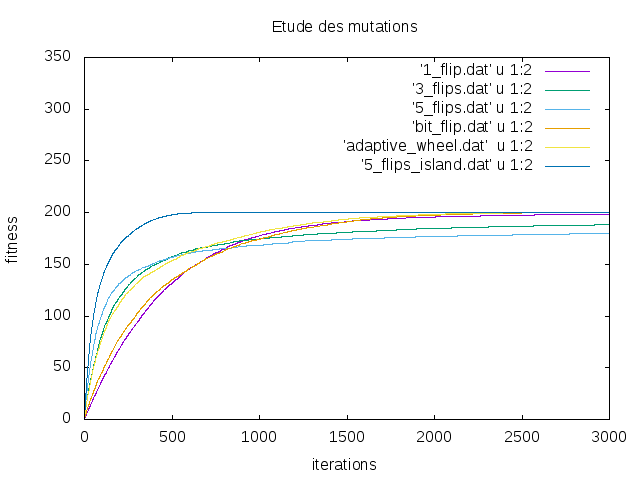
\includegraphics[width=0.5\textwidth]{mutations}{\centering}
    \caption{Les mutations}
    \label{fig:mesh1}
\end{figure}

\item [-] Les croisements:
L'analyse de deux courbes de performances présentées ci dessous permettent de montrer une meilleure efficacité du croisement uniforme. Avec le croisement mono-point, de très bon résultats en termes d'améliorations s'obtiennent que dans le cas ou  les parties récupérées chez chaque individus sont de très bonne qualité. Sinon dans le cas contraire, les résultats sont très peu satisfaisant ou pires. Le croisement permettant de créer une diversité, le choix d'un opérateur permettant de garantir la diversité dans la population a un impact positif sur les performance d'un algorithme génétique.


\begin{figure}[h]
    \centering
    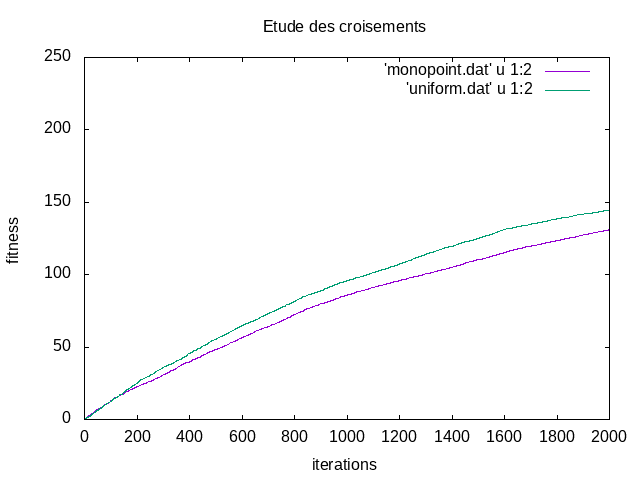
\includegraphics[width=0.5\textwidth]{crossovers}{\centering}
    \caption{Les croisements}
    \label{fig:mesh1}
\end{figure}

\item[-] Les probabilités de mutations:
En faisant varier les probabilités de mutations et notamment avec l'opérateur de mutation N-flips, les 5 courbes présentées ci dessous montrent que de meilleurs résultats s'obtiennent plus rapidement lorsque la probabilité de mutations est plus élevé. Obtenir de meilleurs résultats avec une probabilité moins élevé ou faible nécessite un grand nombre d'itérations. 

\begin{figure}[h]
    \centering
    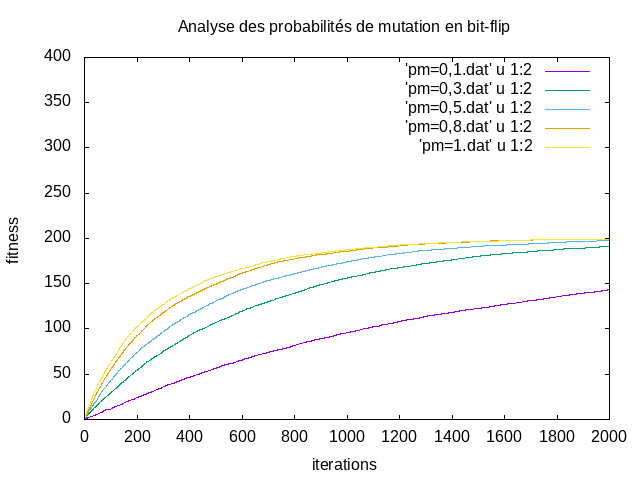
\includegraphics[width=0.5\textwidth]{pm}{\centering}
    \caption{Les probabilités de mutations}
    \label{fig:mesh1}
\end{figure}

\item[-] Les probabilités de croisements:
Contrairement aux opérateurs de mutation (ex: bit-flips) de mutations qui permettent d'obtenir de meilleurs résultats lorsque la probabilité (pm) d'application est plus élevée,  plus la probabilité (pc) est élevée  et moins les résultats sont meilleurs. 
\begin{figure}[h]
    \centering
    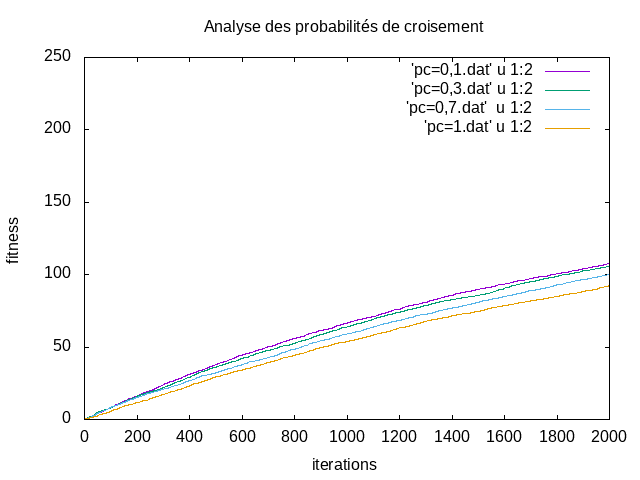
\includegraphics[width=0.5\textwidth]{pc}{\centering}
    \caption{Les probabilités de croisements}
    \label{fig:mesh1}
\end{figure}

\item[-] Les  opérateur de sélections:
Les résultats sont peu satisfaisant lors de l'exécution de l'algorithme avec un opérateur de sélection aléatoire. Les sélections à privilégier sont les méthodes par tournoi ( $k=5$ dans cette étude) ainsi que la sélection par meilleur fitness qui produit de meilleurs résultats.

\begin{figure}[h]
    \centering
    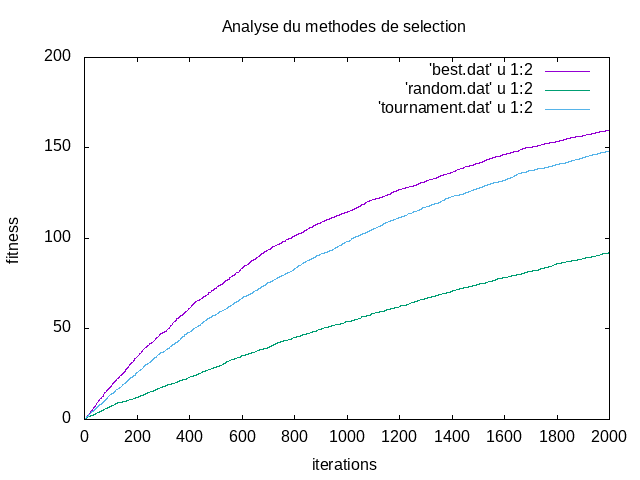
\includegraphics[width=0.5\textwidth]{selections}{\center}
    \caption{les opérateurs de sélections}
\end{figure}

\item[-] L'opérateur d'insertions:
Les deux courbes obtenus montrent que les résultats sont meilleurs avec un mode d'insertion par remplacement des individus les moins bons

\begin{figure}[h]
    \centering
    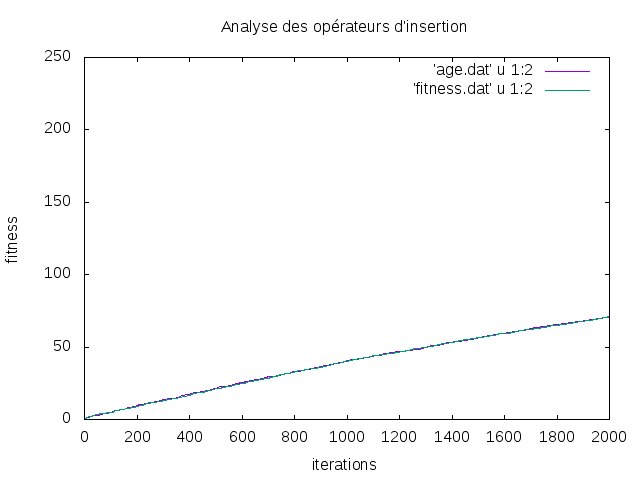
\includegraphics[width=0.5\textwidth]{insertions}{\centering}
    \caption{Les opérateurs d'insertions}
\end{figure}

\end{itemize}

L'étude de ces différentes configurations et leur impact sur la performance de l'algorithme nous permet de proposer deux de cas configurations. La première qualifiée de bonne configuration: sélection des deux meilleurs, croisement uniforme avec faible probabilité pour garantir, faible population, insertion par remplacement des deux moins bons. Concernant les mutations, l'opérateur K-flips avec un K élevé à l'exemple du 5 flips est le bon choix pendant les premières itération de l'algorithme. Un moyen d'éviter la convergence rapide de l'algorithme lors l'opérateur 5-flips serait d'utiliser dans la suite des itérations L'opérateur bits-flip qui réduisent les chances de dégradation et ainsi permet à l'algorithme de converger vers la solution optimale.

\begin{itemize}
\item[-]Application de la sélection adaptative:
Au cours des premières itérations de l'algorithme, les résultats obtenus avec la sélection adaptative d'opérateurs sont meilleurs que ceux des mutations 1-flips et bit-flips se rapprochent en se rapprochant des résultats des mutations 3-flips et 5-flips. Dans la suite des itérations de l'algorithme, la méthode offre de meilleurs  résultats en privilégiant la sélection des opérateurs bit-flips et 1-flips restant ceux qui améliore le plus jusqu'à se rapprocher ou atteindre la solution optimale recherchée.

\item[-]Application des modèles en îles pour l'étude des mutation:
L'opérateur  5 flips tel qu'il présenté dans la figure 3 est peut jugé le  moins  performant des opérateurs suite à la convergence rapide vers un optimum local inférieur à la solution optimal. Mais celui-ci affiche rapidement de meilleurs performances lorsque le modèle en îles est employé.
\end{itemize}

\section{Conclusion}

Cette étude à permis de présenter l'algorithme génétique selon le schéma Steady State. L'analyse des différents composants de l'algorithme et leur impact appliqués sur le problème One-Max  montre l'intérêt du paramétrage si l'on veut arriver à de très bons résultats. La méthode de sélection adaptative d'opérateurs utilisée par la suite dans l'étude des opérateurs mutations cités offre l'avantage d'appliquer chacune des 4 mutations dans les moments où leur probabilité d'amélioration est forte.  ( Model en Iles ...... )


\begin{thebibliography}{9}
\end{thebibliography}
\end{document}
